\documentclass[tikz]{standalone}

\usetikzlibrary{matrix,positioning}
\begin{document}

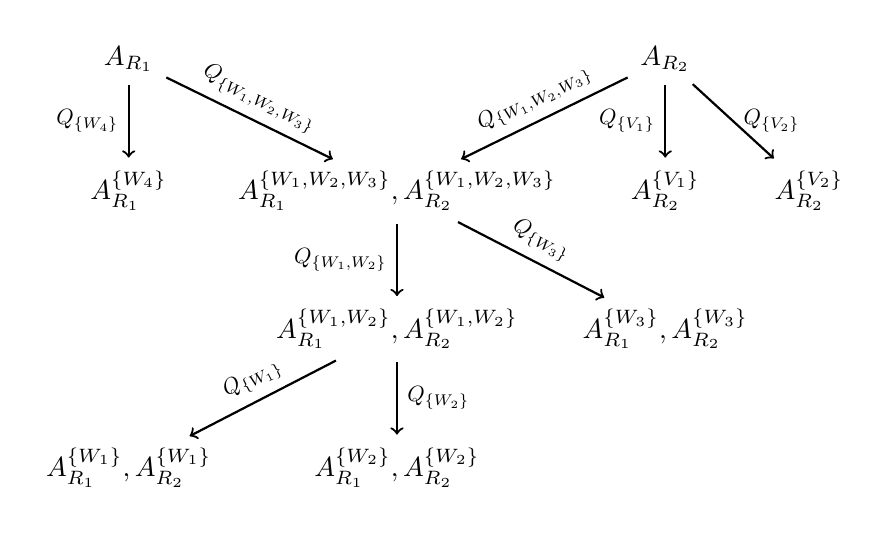
\begin{tikzpicture}[thick,shorten >=1pt, shorten <=1pt,->]
%  \matrix (m) [matrix of math nodes, row sep=3em, column sep={5em,between origins}]{
  \matrix (m) [matrix of math nodes, row sep=2.9em, column sep=0.3em]{
	 A_{R_1} & & A_{R_2} & \\
	A_{R_1}^{\{W_4\}} & A_{R_1}^{\{W_1,W_2,W_3\}},A_{R_2}^{\{W_1,W_2,W_3\}} & A_{R_2}^{\{V_1\}} & A_{R_2}^{\{V_2\}} \\
	& A_{R_1}^{\{W_1,W_2\}},A_{R_2}^{\{W_1,W_2\}} & A_{R_1}^{\{W_3\}},A_{R_2}^{\{W_3\}}\\
	A_{R_1}^{\{W_1\}},A_{R_2}^{\{W_1\}}  & A_{R_1}^{\{W_2\}},A_{R_2}^{\{W_2\}} \\
  };
  \path 
  	(m-1-1) edge node[left] {\scalebox{0.8}{$Q_{\{W_4\}}$}} (m-2-1)
  	(m-1-1) edge node[above right,sloped,anchor=south] {\scalebox{0.8}{$Q_{\{W_1,W_2,W_3\}}$}} (m-2-2)
  	(m-1-3) edge node[above right,sloped,anchor=south] {\scalebox{0.8}{$Q_{\{W_1,W_2,W_3\}}$}} (m-2-2)
  	(m-1-3) edge node[left] {\scalebox{0.8}{$Q_{\{V_1\}}$}} (m-2-3)
  	(m-1-3) edge node[right] {\scalebox{0.8}{$Q_{\{V_2\}}$}} (m-2-4)
  	(m-2-2) edge node[left] {\scalebox{0.8}{$Q_{\{W_1,W_2\}}$}} (m-3-2)
  	(m-2-2) edge node[right,sloped,anchor=south] {\scalebox{0.8}{$Q_{\{W_3\}}$}} (m-3-3)
  	(m-3-2) edge node[left,sloped,anchor=south] {\scalebox{0.8}{$Q_{\{W_1\}}$}} (m-4-1)
  	(m-3-2) edge node[right] {\scalebox{0.8}{$Q_{\{W_2\}}$}} (m-4-2)
  ;
\end{tikzpicture}
\end{document}